\chapter{Implementation}
\label{impl}


We now describe the implementation details of each component in \name.
We implemented a prototype that comprises a software-based gateway and controller.
The main development language is \fnurl{golang 1.14.1}{https://golang.org/doc/go1.14}, and we used \fnurl{SQLite3}{https://www.sqlite.org/releaselog/3_32_0.html} for the database. To secure control-plane channels, we also leveraged
\fnurl{TLS 1.3}{https://tools.ietf.org/html/rfc8446}. The prototype is publicly \fnote{available}{\url{https://github.com/chaehni/scion/tree/zoning}}.

Our implementation builds on top of the SCION architecture~\cite{Perrig2017}.
The implementation decision has been driven by the following reasons: i) SCION
provides network programmability along with the separation of control and data
plane, ii) SCION comes with an embedded PKI system that can be utilized for our
key management system, and iii) the open source version of the
\fnurl{DRKey}{https://github.com/netsec-ethz/scion/tree/scionlab_previousversion/go/lib/drkey}
system as well as a software-based gateway working with SCION are available,
thus enabling rapid prototyping.


\section{Translation Point}
\label{sec:tp}

To implement a prototype of \tp, we extend the \fnurl{SCION-IP Gateway (SIG)}{https://github.com/scionproto/scion}.
The main functionality of SIG is to encapsulate legacy IP packets into SCION packets and
vice versa. In this context, a SIG acts as a gateway between an internal (legacy) network
and an external (SCION) network. Since \tp is designed as a gateway that bridges LAN
traffic over WAN---the underlying inter-domain routing protocol is not relevant here---the
functional aspects of \tp meets with what SIG provides. To be integrated with SIG, \tp
mediates between the UNIX socket and SIG socket, and performs zone transfer authorization
and verification for all incoming/outgoing packets.

\subsection{Modular Design}
\label{ssec:mod_design}

\paragraph{Packet Format}
In order to make \tps modular, all modules must agree on a common packet format on which they
operate. The packet contains the raw IP packet read from the interface, as well as metadata
that is required by the modules to perform their task. Modules can read and write all fields of the
packet. In particular they can modify the raw IP packet.
Listing~\ref{lst:packet} shows the packet format.

\begin{minipage}{\linewidth}
	\begin{lstlisting}[
		basicstyle=\footnotesize, language=golang,
		caption={The abstract packet format passed between the modules of a \tp.},
		label=lst:packet,
	]
	// Packet contains a raw IP packet with additional meta data
	type Packet struct {
		Ingress		bool
		SrcHost 	net.IP
		DstHost 	net.IP
		RemoteTP	string
		DstZone		uint32
		RawPacket 	common.RawBytes
	}
	\end{lstlisting}
\end{minipage}

The \code{Ingress}field identifies a packet as either an ingress packet,
coming from the WAN, or an egress packet
that originated in the local network. \code{SrcHost} and \code{DstHost} reflect
the source and destination IP addresses of the packet. \code{RemoteTP} designates
the remote \tp. For an ingress packet that is the source \tp from which the packet
was received, for an egress packet it is the \tp to which the packet needs to be
forwarded to. \code{DstZone} is the Zone ID of the zone to which \code{DstHost}
belongs.

\paragraph{Module Interface}
A module is then simply defined as a type that handles this packet format.
More precisely, a module implements a very simple \code{Module} interface.

\begin{minipage}{\linewidth}
	\begin{lstlisting}[
		basicstyle=\footnotesize, language=golang,
		caption={The interface all modules must implement.},
		label=lst:module,
	]
	// Module is a single element in the pipeline
	// that handles IP packets.
	// Modules must be thread safe.
	type Module interface {
		Handle(Packet) (Packet, error)
	}
	\end{lstlisting}
\end{minipage}

As can be seen in Listing~\ref{lst:module}, modules call \code{Handle} to process packets
of the aforementioned format and then return a new, potentially modified, packet and an
error. The error is \code{nil} if the handling of the packet was successful.

\paragraph{Handler Chains}
\label{ssec:chains}

Modules can be linked in a specific order to create a chain of handlers.
These handler chains can then be registered for a specific use case. In particular, it is possible
to create different handler chains for intra-domain and inter-domain zone transfers.

\subsection{Implemented Modules}
\label{ssec:modules}

\begin{figure}[htb]
	\begin{center}
		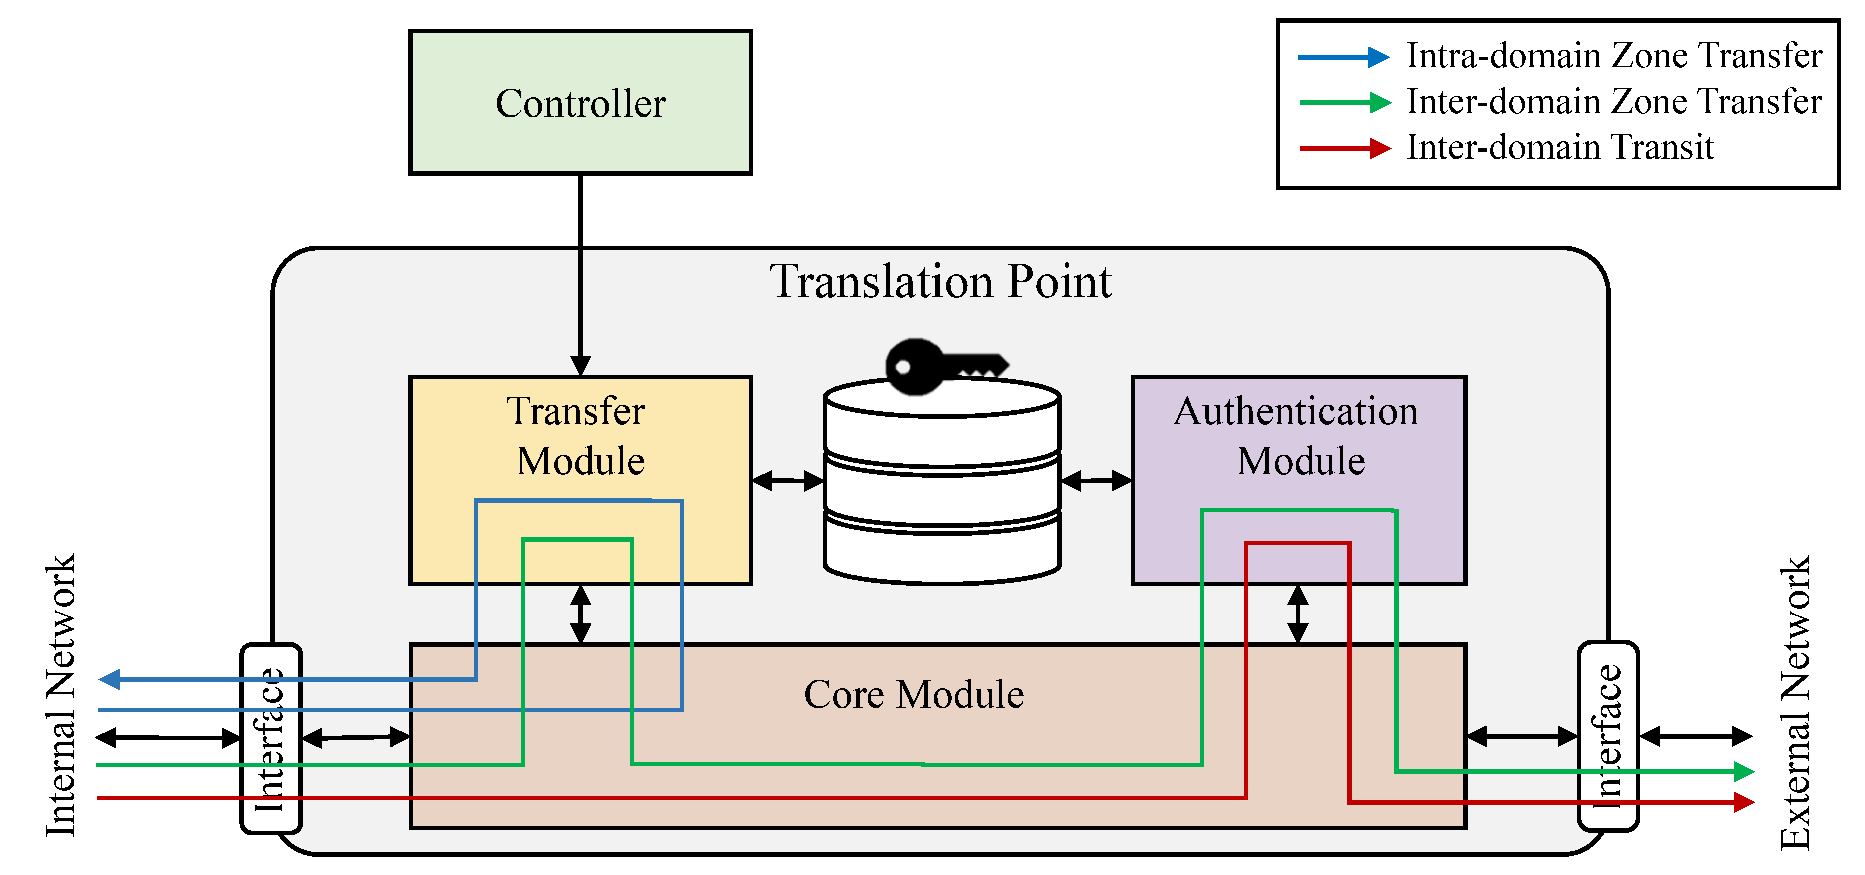
\includegraphics[width=0.9\textwidth]{tp.eps}
	\end{center}
	\caption{An overview of the modularized \tp implementation. Major use cases are
	indicated with colored arrows.}
	\label{fig:tp}
\end{figure}

In this section we describe the main modules that have been implemented to satisfy
the protocol described in \S\ref{sec:protocol}. Figure~\ref{fig:tp} illustrates
the implementation details of the modularized \tp design that consists of the three
main modules: i) core module, ii) transfer module, and iii) authentication module.

\paragraph{Core Module}
The core module is the main loop of \tp. It reads packets from the UNIX socket and
redistributes them to the corresponding interfaces. More precisely, when receiving packets
from the internal network, it retrieves metadata such as source and destination
IP addresses (as illustrated in
\S\ref{ssec:mod_design}) from the raw packet and hands over to the transfer module.
If the zone transfer is authorized ($return=1$),
the packet is then either forwarded back to the internal network or, in case the given destination
is in a remote zone,
once again handed over to the authentication module to be prepared for secure transmission.
For packets coming from the external network, a \tp first calls the authentication module for
verification of the conveyed authentication token. Packets with invalid tokens are simply discarded.

\paragraph{Transfer Module}
The main objective of this module is to check the zone transfer rules. The transfer
module communicates with its controller to maintain a list of up-to-date zone transfer policies.
To this end, it establishes a TLS channel with the controller, downloads policies,
and populates the database.
We implemented the transfer module to support different drop-in options using APIs.

\begin{itemize}
	\item No-Op: This is for a setup in which no inter-domain zone transfers are required,
	      but only inter-domain zone extensions.
	\item Standard: This mode would perform an authorization check for the requested
	      zone transfer based on the source and destination IP addresses.
	\item Firewall: If needed, the module could be instantiated as a full-fledged firewall.
	      This mode would be useful for cases where the firewall can not be replaced.
\end{itemize}

While the No-Op and Firewall options are both trivial to implement (the first simply accepts all
packets while the latter forwards packets to the firewall instance), it is crucial for the Standard
option to efficiently match IP addresses against a list of trusted IP subnets. In our implementation
we leverage a compressed trie data structure (also radix trie or compact prefix tree) to check if a
given pair of source and destination IP addresses are allowed to exchange data. Specifically,
we use the open source \fnurl{cidranger}{https://github.com/yl2chen/cidranger} library. Since the
lookup time of the trie is only dependant on the depth of the trie, which is fixed (32 bits for IPv4 and 128
bits for IPv6), the lookup time is constant with respect to the number of stored subnets. This
ensures fast packet processing even if a \tp has a large number of rules configured.
Figure~\ref{fig:trie} shows a simplified example of how a trie stores IP subnets.

\begin{figure}[htb]
	\begin{center}
		\includegraphics[width=0.9\textwidth]{trie.pdf}
	\end{center}
	\caption{The first few levels of a trie storing the subnets 128.0.0.0/3, 160.0.0.0/4, and 224.0.0.0/4.}
	\label{fig:trie}
\end{figure}

While the trie stores all configured IP subnets known to the \tp, another data structure is required
to store the actual zone transfer rules, stating which zones, and by extension which subnets, are
allowed to communicate with each other---recall that a subnet corresponds to exactly one zone. For this,
we use a fast in-memory key-value store which maps to a given zone all other zones from which it
accepts traffic.

\paragraph{Authentication Module}
For inter-domain packet transmissions, the authentication module issues
authentication tokens (further discussed in \S\ref{sec:token}) for outgoing packets.
It (ideally) caches the first-level keys prefetched
from other \tps and derives a second-level key to generate the authentication token. Inversely, for
packets incoming from other \tps, it derives the corresponding 2nd-level key
and verifies the attached authentication token. The authentication module is in itself modular by
relying on an interface to fetch and derive keys. The key management logic, which is
responsible for exchanging, caching, and evicting expired keys, is completely
decoupled from the rest of the module. This has the advantage that the key exchange protocol can be changed
independently, without a need to modify other parts of the module. The interface that all
implementations of such a key manager must satisfy is depicted in Listing~\ref{lst:keyman}.

\begin{minipage}{\linewidth}
	\begin{lstlisting}[
	basicstyle=\footnotesize, language=golang,
	caption={The KeyManager interface used by the authentication module to fetch and
	derive keys.},
	label=lst:keyman,
]
// KeyManager is a thread-safe key store managing L0 and L1 keys
type KeyManager interface {
	// FetchL1Key fetches the level 1 key to be used to send
	// data to remote. It returns the key and a bool
	// indicating if the cached key was expired and a fresh
	// key has been fetched from remote.
	FetchL1Key(remote string) ([]byte, bool, error)
	// FetchL2Key fetches the Level-2 key used to encrypt
	// outgoing traffic
	FetchL2Key(remote string, zone uint32) ([]byte, bool, error)
	// Derive L1Key derives the level 1 key used to derive
	// the L2 key.
	DeriveL1Key(remote string) ([]byte, error)
	// Derive L2Key derives the level 2 key used to verify
	// incoming traffic.
	DeriveL2Key(remote string, zone uint32) ([]byte, error)
}
	\end{lstlisting}
\end{minipage}

\section{Controller}
\label{sec:controller}

We implemented the controller as a Web server written in golang with an SQLite database storing the
zone information and transfer policies. The controller offers an API which allows
\tps to fetch zoning information via HTTPS GET requests.

\paragraph{APIs}
The endpoints of interest are:

\begin{enumerate}
	\item \code{/api/get-subnets}
	\item \code{/api/get-transfers}
\end{enumerate}

Using these endpoints \tps fetch IP subnet and zone transfer rules. Important
to note is that the controller only hands out the subset of the full set of rules
which is required for the requesting \tp to be operational. This minimizes the size
of data transmissions and also improves security by not disclosing the full network
view to every \tp. For every call to the API the controller first verifies the
authenticity of the caller before the request is forwarded to the corresponding
handler. The handlers then load the requested data from the database and send it to
the caller as JSON-formatted bytes.

\begin{minipage}{\linewidth}
	\begin{lstlisting}[
		basicstyle=\footnotesize, language=golang,
		caption={Abstraction layer function that inserts zone transfer rules into the database.},
		label=lst:subnets,
	]
// InsertTransfers inserts premitted zone transfers into the backend
func (b *Backend) InsertTransfers(transfers types.Transfers) error {
	stmt := `INSERT INTO Transfers (src, dest) VALUES (?, ?)`

	// do insertion in a transaction to ensure atomicity
	tx, err := b.db.BeginTx(context.Background(), nil)
	if err != nil {
		return err
	}

	for src, dests := range transfers {
		for _, dest := range dests {
			_, err = tx.Exec(stmt, src, dest)
			if err != nil {
				tx.Rollback()
				return err
			}
		}
	}
	tx.Commit()
	return nil
}
	\end{lstlisting}
\end{minipage}

\paragraph{Database}
The database consists of four tables (Zones, Sites, Subnets, Transfers), each describing one of
the core elements of the architecture.
The database schema is listed in Appendix~\ref{apdx:controllerdb}. An abstraction layer
written in golang allows the controller to interface with the database using high-level calls.
The abstraction layer makes use of transactional queries to ensure consistency even in the event
of errors. Furthermore, the abstraction uses prepared statements for insertions, deletions and
retrievals of data. This protects against SQL-injections and improves the speed of queries.
An example function of the abstraction layer is depicted in Listing~\ref{lst:subnets}.

\section{Authentication Token}
\label{sec:token}

\begin{figure}[htb]
	\begin{center}
		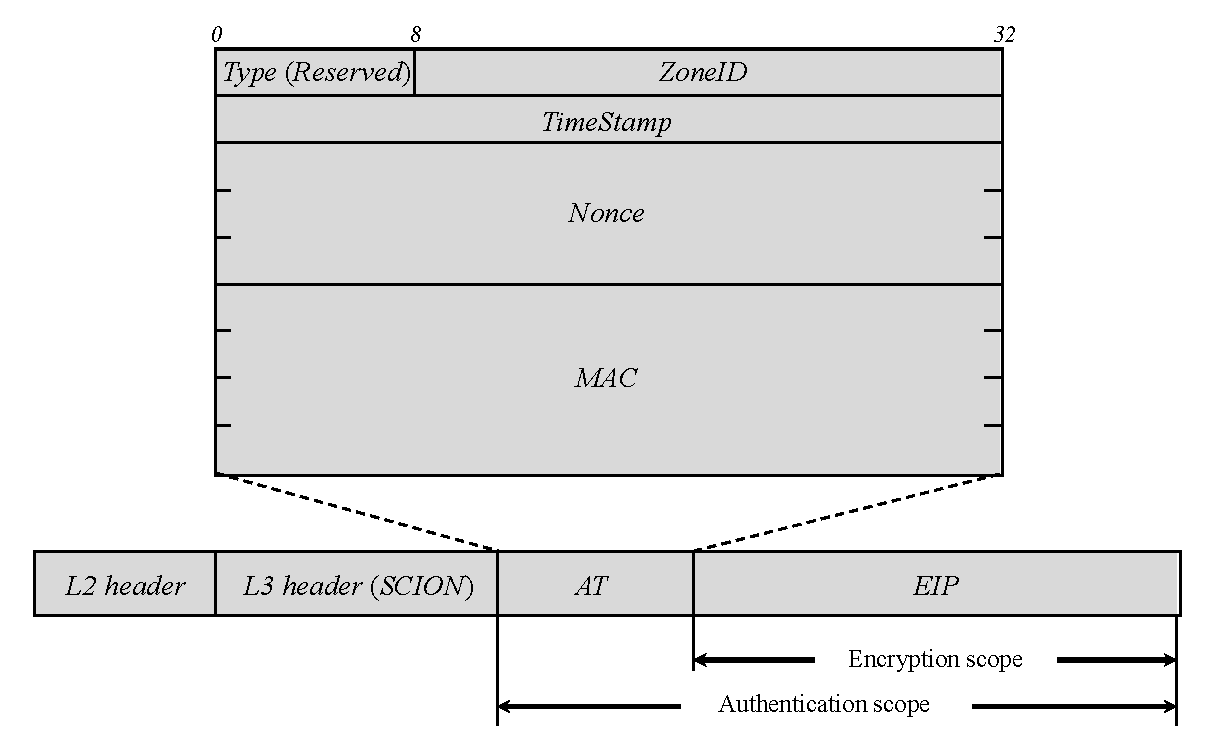
\includegraphics[width=.9\textwidth]{header.eps}
	\end{center}
	\caption{\name packet format for secure tunneling.}
	\label{fig:header}
\end{figure}

The \name packet format follows the IP tunneling conventions of encapsulating the original
packet with a new outer IP header that indicates the two tunnel endpoints as the new source
and destination. The original packet is encrypted and then authenticated along with the new
packet header fields. Figure~\ref{fig:header} shows the detailed packet structure and coverages
of the confidentiality and integrity guarantee.

The authentication token starts with one byte of reserved space for a \textit{Type} field. While
currently unused this will be useful in the future for distinguishing different variations of
the authentication token. \textit{ZoneID} depicts the 3 byte long zone identifier of the
destination zone. It is used by the receiving \tp to derive the correct key for MAC verification
and decryption. The next 4 bytes are occupied by a \textit{TimeStamp} which is added by the
sending \tp. It is the Unix time at the point of sending the packet. The receiving \tp uses this
timestamp to reject replayed packets. The timestamp is followed by a \textit{Nonce} of 12 bytes.

The nonce as well as the previous three token fields and the data to be encrypted (\textit{EIP})
serve as input to a \textit{Galois/Counter Mode} (GCM) algorithm with an underlying
\textit{AES-128} block cipher as cryptographic primitive. This mode of operation is widely
adopted for its performance as well as the capability to do \textit{authenticated encryption
with associated data} (AEAD). Here it provides authenticity over the header fields
(\textit{Type}, \textit{ZoneID}, \textit{TimeStamp}) and the data in \textit{EIP} while
\textit{EIP} additionally also gets encrypted.

The 16 byte \textit{MAC} generated by GCM is the last field in the authentication token. Both,
the nonce and the MAC sizes follow the guidelines recommended by NIST SP 800-38D \cite{nistgcm}.

Listing~\ref{lst:transformer} shows the interface that is used by the authentication module
to create and attach an authentication token to an IP packet. Of particular interest are the
functions \code{ToIR} and \code{FromIR}. \code{ToIR} takes the raw
\code{packet}, a \code{key} and some metadata (\code{remote}, \code{dstZone}) and returns the
encrpyted packet with attached tag and an error. The error is \code{nil} if the
call was successful.
Inversely, \code{FromIR} receives an encrypted packet with attached token (\code{cipher}) and
a \code{key} and then returns the decrypted \code{packet} together with the token (\code{additionalData})
and an error. The error is again \code{nil} if the
call to the function was successful.

\begin{minipage}{\linewidth} % minipage makes the listing unsplittable
	\begin{lstlisting}[
		basicstyle=\footnotesize, language=golang,
		label={lst:transformer},
		caption={The Transformer interface used by the authentication module 
		to create and verify authentication tokens.},
	]
	// Transformer transforms IP packets to and from intermediate
	// representation
	type Transformer interface {
		// ToIR transforms packet to intermediate
		// representation.
		ToIR(remote string, key, packet []byte, dstZone uint32)
			([]byte, error)
		// FromIR transforms cipher from intermediate representation
		// back to a regular IP packet
		FromIR(key, cipher []byte)
			(additionalData []byte, packet []byte, err error)
		// ResetState resets the nonce state for remote	
		ResetState(remote string) error
		// GetZone retrieves the zoneID encoded in token
		GetZone(token []byte) (uint32, error)
	}
	\end{lstlisting}
\end{minipage}

If the token format needs to be changed, only the implementation of the \code{Transformer} interface
needs to be modified. The rest of the module can remain unchanged.
